\chapter{Related work} % Main chapter title

\label{Chapter2} % Change X to a consecutive number; for referencing this chapter elsewhere, use \ref{ChapterX}


%----------------------------------------------------------------------------------------
%	SECTION 1
%----------------------------------------------------------------------------------------
\section{Haptic Feedback in VR}
Haptic feedback is a technology that provides tactile sensations to users, enabling them to physically feel virtual objects and interactions. In virtual reality, the lack of touch feedback can limit realism and diminish the sense of presence. To address this limitation, haptic feedback systems are integrated alongside visual and auditory cues, resulting in a richer and more immersive user experience. Haptic feedback allows users to perceive various object properties, such as texture, shape, stiffness, and temperature, which would otherwise be absent in digital environments~\cite{doi:10.34133/research.0333}.

\subsection{Vibrotactile Feedback}
Vibrotactile feedback is one of the most commonly used haptic methods in virtual reality, especially in wearable applications. This technique employs small vibrating actuators to create tactile sensations on the skin, enabling users to experience interactions such as contact with virtual objects, collision effects, surface textures, and environmental cues. Its popularity is due to several advantages, including compact size, low cost, energy efficiency, fast response times, and ease of integration into various wearable devices, such as gloves, vests, thimbles, and headgear.

Research consistently demonstrates that vibrotactile feedback effectively enhances user immersion. For instance, a study by Barsen et al.~\cite{10.1007/978-3-030-06134-0_25} on commercial VR systems equipped with vibrotactile vests revealed that participants reported significantly higher levels of co-presence and realism when vibrotactile cues were present during avatar collisions. Additionally, a review by H. Shiying~\cite{10.54254/2753-8818/17/20240650} confirmed that vibrotactile stimulation effectively conveys fine textures and surface variations, making it particularly suitable for VR texture-rendering tasks.

\newpage
\subsection{Force Feedback}
Force feedback is a key haptic technology that creates mechanical resistance to mimic the physical characteristics of virtual objects, such as weight, stiffness, and collision forces. This technology typically uses motors, gears, or mechanical linkages to generate opposing forces in response to user movements, enhancing the realism of physical interactions within virtual environments. Force feedback is commonly found in haptic exoskeleton gloves, joystick-based systems, and haptic robotic arms. It is particularly valuable in training simulators, rehabilitation, and virtual manipulation tasks where a realistic sense of force is essential.~\cite{10.3389/fbioe.2020.541105}

Numerous studies have shown that force feedback significantly improves user interaction and realism in virtual environments. Zhang et al.~\cite{zhang2025doglovedexterousmanipulationlowcost} introduced the DOGlove, a low-cost, open-source glove that provides five degrees of freedom (5-DoF) force feedback at the fingertips. This is achieved through compact, cable-driven torque systems, which enable high precision in teleoperation and underscore the crucial role of force feedback in contact-intensive robotic manipulation.

\subsection{Thermal Feedback}
Thermal feedback conveys sensations of temperature—whether warmth or coolness—through haptic interfaces, which enhances the realism of materials in virtual reality environments. By simulating the thermal properties of objects, users can distinguish virtual materials not only by touch but also by temperature, leading to more immersive interactions. Thermal actuators typically utilize Peltier thermoelectric elements or resistive heating pads, enabling dynamic temperature modulation in response to various virtual scenarios~\cite{TANG2024100365}.

Kang et al.~\cite{10.48550/arXiv.2405.11807} developed a dual-sided rotating Peltier module system that facilitates quick transitions between warm and cool stimuli, which is perfect for real-time VR applications. This system also enhances user comfort through the use of layered insulation.

%----------------------------------------------------------------------------------------
%	SECTION 2
%----------------------------------------------------------------------------------------
\newpage
\section{Texture Rendering}
Texture rendering in virtual reality aims to replicate the tactile sensations of various materials to create a realistic perception of surface properties. This process involves multiple sensory channels, including visual, auditory, and haptic feedback. Research consistently demonstrates that haptic feedback is crucial for authentic texture perception, especially in interactive VR applications. The objective of texture rendering is to enable users to identify and differentiate between virtual surfaces as naturally as they would with physical surfaces. This capability significantly enhances the sense of presence, immersion, and realism in VR environments.
\begin{figure}[H]\centering
	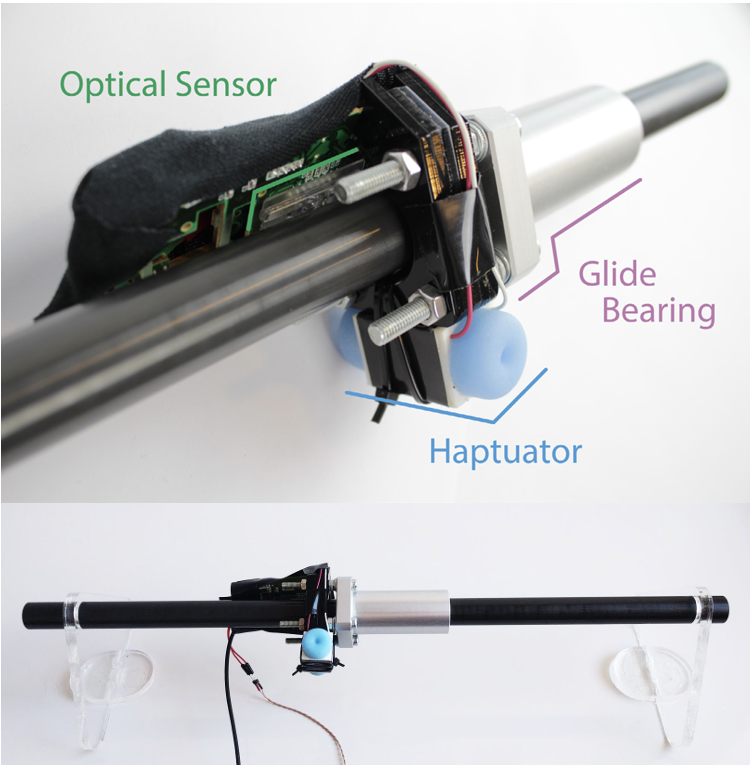
\includegraphics[width=0.6\textwidth]{Pictures/Texture_Rendering_1.png}%imagine location
	\caption{Slider used for experiment. Participants interact with slider by moving the silver glide bearing~\cite{10.1145/3025453.3025812}}\label{fig:Texture_Rendering_1}%use name for ref.
\end{figure}

P. Strohmeier et al. ~~\cite{10.1145/3025453.3025812} proposed a method for generating haptic textures by integrating vibrotactile feedback with user movement. Their approach is based on the idea that texture perception in real-world interactions arises from active exploration, with vibrations produced by the relative motion between the finger and the surface. To simulate this mechanism, they developed a custom haptic interface, as shown in Fig.~\ref{fig:Texture_Rendering_1}. This interface incorporates a linear slider, a BM3C Haptuator, an optical position sensor, and features minimal mechanical friction to avoid interference from passive forces.

The study explored four dimensions of perceptual texture: roughness, bumpiness, sharpness, and adhesiveness. These dimensions are consistent with established theories of tactile perception~~\cite{6216375}.The authors systematically varied three key vibrotactile parameters(Fig.~\ref{fig:Texture_Rendering_2}): granularity, amplitude, and timbre. Participants took part in a magnitude estimation task, where they rated the intensity of perceived textures based on different configurations of these parameters. The results revealed that granularity was the primary factor in distinguishing between textures in terms of roughness and bumpiness.

\begin{figure}[H]\centering
	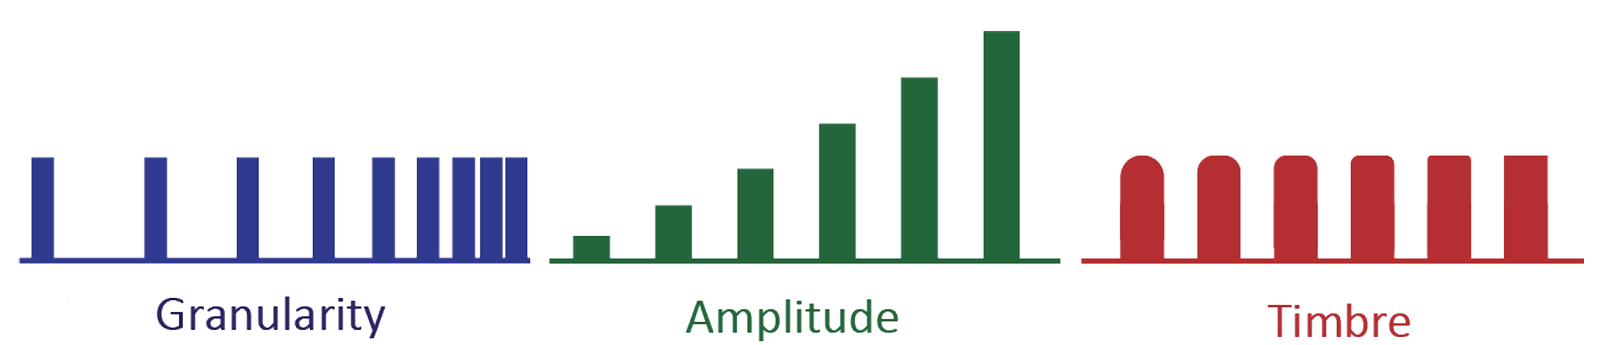
\includegraphics[width=1\textwidth]{Pictures/Texture_Rendering_2.png}%imagine location
	\caption{Naïve visualization of vibrotactile parameters~\cite{10.1145/3025453.3025812}}\label{fig:Texture_Rendering_2}%use name for ref.
\end{figure}

%----------------------------------------------------------------------------------------
%	SECTION 3
%----------------------------------------------------------------------------------------

\section{Research Gap and Positioning of This Work}
Previous studies in the field of haptic feedback for virtual reality have explored various methods to enhance tactile realism. Force-feedback systems provide mechanical resistance, allowing users to feel weight and stiffness. However, these systems are often bulky, complex, and can hinder mobility, making them unsuitable for lightweight wearable applications. Thermal feedback has also been used to simulate directionality and temperature cues, but it suffers from slow response times and limited surface coverage. In contrast, vibrotactile feedback has emerged as the most common approach due to its simplicity, low cost, and responsiveness. However, many studies still rely on amplitude or frequency modulation to represent contact events and basic textures.

This study, however, takes a different approach by focusing on cycle rate modulation using pulse-width modulation to convey the roughness and bumpiness of textures. Instead of modifying vibration amplitude or frequency, which often requires precise tuning of actuators, our method alters the rhythm (on-off timing) of vibration pulses to represent texture properties. This approach offers several practical advantages: it enables the use of a single actuator per finger, eliminates the need for complex multi-actuator arrays, and reduces hardware complexity while still producing clearly distinguishable tactile sensations associated with surface roughness and bumpiness. 

Furthermore, by relying solely on PWM cycle rate modulation, the system simplifies both hardware implementation and software control, making it particularly suitable for lightweight and real-time VR applications.

